\chapter{Анализ}\label{ch:ch2}

\section{Среда выполнения}\label{sec:ch2/sec1}

Проанализировав требования к среде выполнения, были представлены следующие варианты реализации:
\begin{enumerate}[beginpenalty=10000] % https://tex.stackexchange.com/a/476052/104425
  \item Собственная реализация среды на основе микросервисной клиент-серверной архитектуры;
  \item Использование стороннего фреймворка Robot Operating System (ROS).
\end{enumerate}

\subsection{Собственная реализация}
В качестве вариант рассматривалась собственная реализация среды выполнения на основе микросервисной архитектуры, включающая в себя следующее: 
\begin{enumerate}[beginpenalty=10000] % https://tex.stackexchange.com/a/476052/104425
  \item Сервер - хранилище сообщений от микросервисов. В его обязанности будут входить: приём, передача, согласование формата сообщений, удаление устаревших данных.
  \item Сами микросервисы. Помимо их основной работы, они должны принимать с сервера входные данные и отправлять выходные данные для последующей работы остальных сервисов.
\end{enumerate}

Схема представленного варианта изображена на Рисунке~\cref{fig:microservice}.

\begin{figure}[ht]
    \centerfloat{
        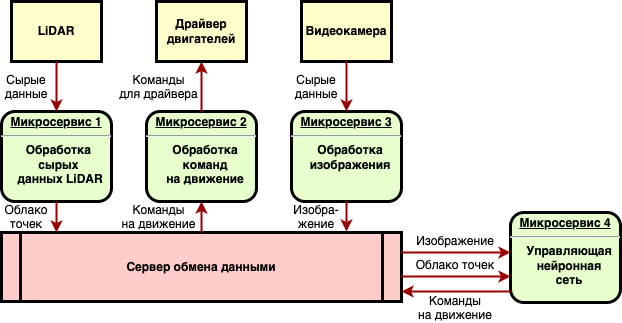
\includegraphics[scale=0.7]{microservice}
    }
    \caption{Пример архитектуры собственной реализации среды выполнения для робота на основе микросервисной архитектуры}\label{fig:microservice}
\end{figure}

Данный вариант был отвергнут в следствии существования более быстрого и удобного варианта реализации, описанного в следующей секции.

\subsection{Фреймворк Robot Operating System}
Robot Operating System или сокращённо ROS предоставляет удобные и мощные функции, помогающие разработчикам в таких задачах, как передача сообщений различного типа, распределение вычислений между компьютерами, повторное использование кода и реализация современных алгоритмов для роботов~\cite[с.~7]{ros}. В общем случае, ROS представляет собой инструмент, позволяющий связывать несколько независимых программных модулей при
помощи сервисов и узлов, которые могут передавать друг другу сообщения в различном формате. Структура ROS представлена на Рисунке~\cref{fig:ros-struct}~\cite[с.~19]{ros}.

\begin{figure}[ht]
    \centerfloat{
        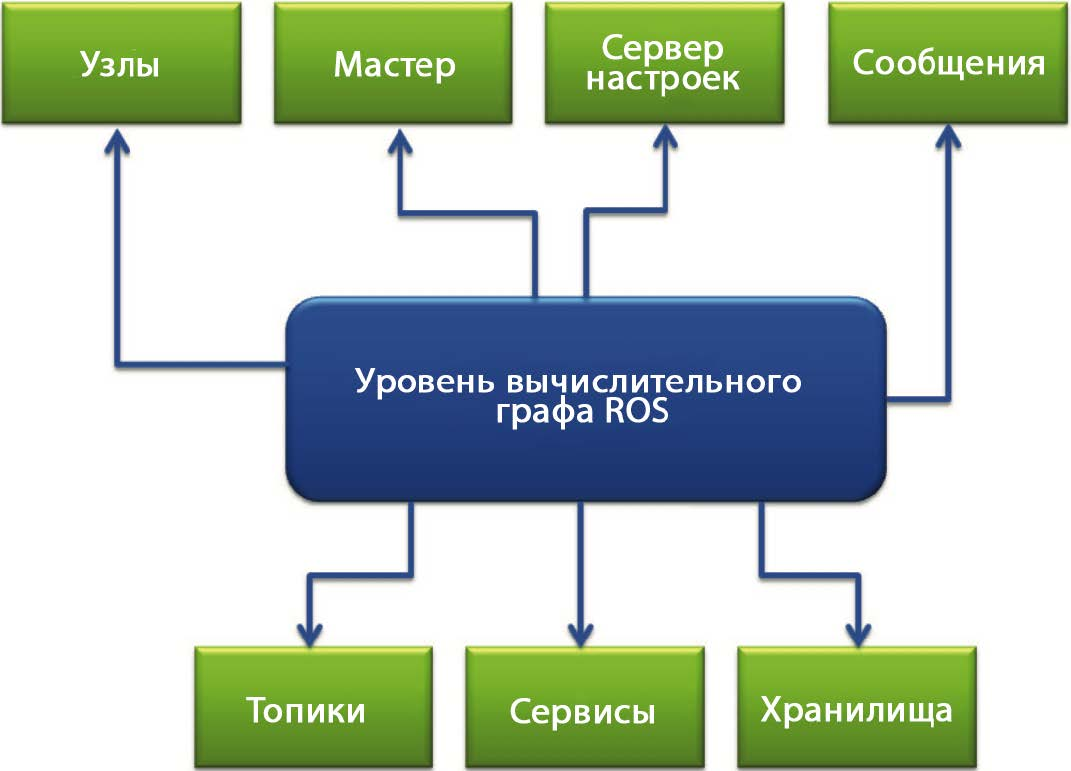
\includegraphics[scale=0.9]{ros-struct}
    }
    \caption{Общая структура Robot Operating System}\label{fig:ros-struct}
\end{figure}

Большими преимуществами использования данного фреймворка является возможность передачи сообщений по локальной сети и обширная библиотека уже реализованного ПО, которое можно без относительно больших затрат по времени интегрировать в свой собственный проект. На момент написания данной работы глобальный репозиторий ROS Index насчитывает 2455 подключенных к нему сторонних репозиториев и 6927 пакетов. Диаграмму соответствия пакетов в репозитории с версиями ROS\footnote{Версия, используемая в данной работе - ROS Melodic} можно увидеть на Рисунке~\cref{fig:ros-repo}~\cite{ros-repo}.

\begin{figure}[ht]
    \centerfloat{
        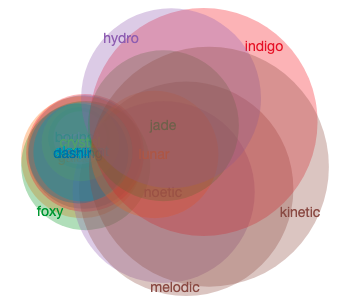
\includegraphics[scale=0.7]{ros-repo}
    }
    \caption{Диаграмма соответствия глобального репозитория ROS Index и версий ROS}\label{fig:ros-repo}
\end{figure}

\subsubsection{Концепции ROS}
Ниже приведён список концепций рассматриваемого фреймворка:

\begin{itemize}[beginpenalty=10000] % https://tex.stackexchange.com/a/476052/104425
  \item \textbf{Узел} --- это процесс, выполняющий вычисления. Каждый узел написание с использованием клиентских библиотек ROS. Используя методы связи, узлы могут общаться друг с другом заранее определённым форматом сообщений и обмениваться данными. Для этого создаются узлы-подписчики, и узлы-публикаторы;
  \item \textbf{Мастер} --- обеспечивает регистрацию и работоспособность запущенных узлов;
  \item \textbf{Сообщение} --- простая структура данных, содержащая типизированное поле, которое может содержать целый набор данных, отправляемых на другой узел. Помимо стандартных типов сообщений\footnote{Такие как целые числа, с плавающей точкой, логический тип, строковый...} возможна отправка заранее обозначенных собственных типов сообщений;
  \item \textbf{Топик} --- именованная шина данных, используемая узлами для отправки сообщений. Публикующий и подписанный узел не знают о существовании друга друга. Благодаря тому, что каждый топик имеет уникальное имя, любой узел может получить доступ к данному топику и отправляет через него данные, при условии соблюдении заранее оговорённых передаваемых типов, данным топиком;
  \item \textbf{Сервисы} --- реализация удалённого вызова процедур\footnote{RPC} в ROS. В некоторых случаях модель связи публикации и подписки может не
подходить. В этих случаях и применяют взаимодействия в виде сервисов (схема запрос/ответ), при котором один узел может запросить выполнение процедуры для другого узла, ожидая какого-то обязательного ответа\footnote{В случае использования схемы с подписчиками и публикаторами доставка сообщений и ответ
не гарантируются}~\cite[с.~20]{ros}.
\end{itemize}

\section{Обеспечение необходимых данных}
\subsection{Информация об окружающем пространстве}
Для предоставления информации об окружающем пространстве в режиме реального времени со всех сторон робота было принято решение об установке прибора лазерного сканирования, реализующего технологию LiDAR. Такое устройство представляет собой дальномер оптического диапазона, который замеряет угол и расстояние до точки, получая таким образом полярные координаты.

Существует два основных типа LiDAR'ов:

\begin{enumerate}[beginpenalty=10000] % https://tex.stackexchange.com/a/476052/104425
  \item 3D LiDAR;
  \item 2D LiDAR.
\end{enumerate}

Первый позволяет получить 3D картинку. Обычно такой LiDAR оснащён подвижным лазером, который довольно долго сканирует перед собой окружающую местность. Однако, уже сейчас можно найти 3D LiDAR, которые сканируют с довольно быстрой скоростью~\cite[с. 308]{lidar-3d}. Примером результата такой работы может стать картинка, изображённая на Рисунке~\cref{fig:lidar-3d}. На сегодняшний день такие LiDAR'ы являются довольно дорогими устройствами.

\begin{figure}[ht]
    \centerfloat{
        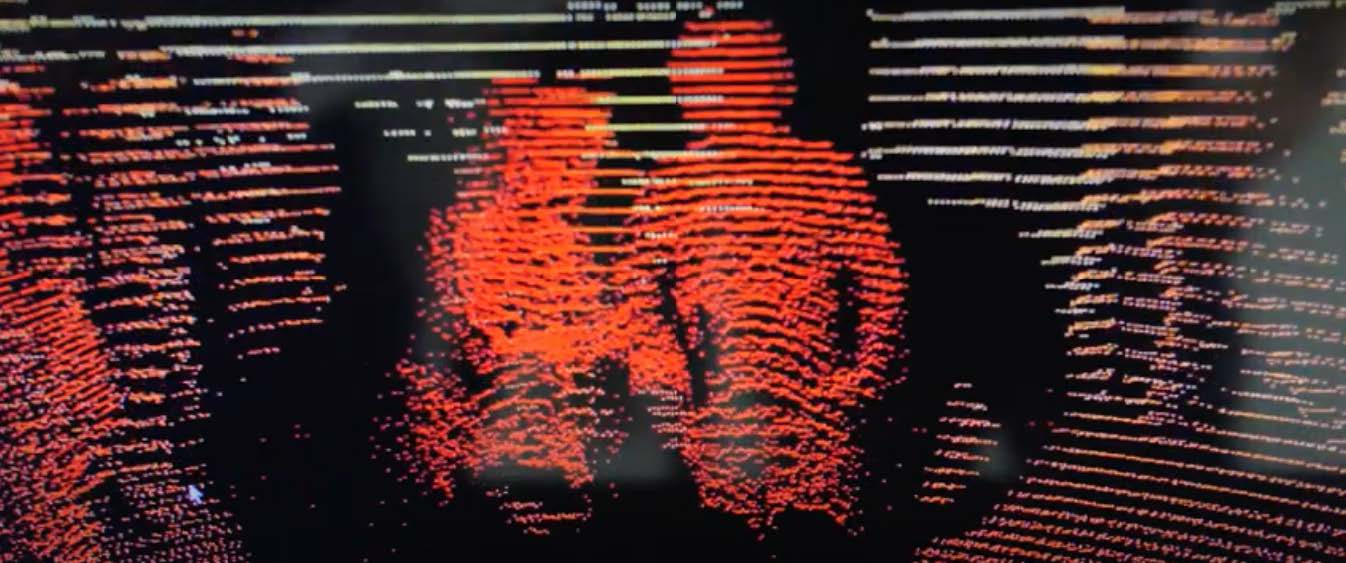
\includegraphics[scale=1.0]{lidar-3d}
    }
    \caption{Пример визуализации данных 3D LiDAR'а, представленном на выставке CEATEC 2017 компанией Panasonic Японии}\label{fig:lidar-3d}
\end{figure}

Второй, соответственно, создаёт двухмерное облако точек, которое также можно визуализировать в виде картинки, пример которой изображён на Рисунке~\cref{fig:lidar-2d}. Такой LiDAR обычно сканирует область вокруг себя и имеет угол обзора 360 градусов. Лазер также является подвижным, но только в этот раз он просто движется вокруг своей оси~\cite[с. 610]{lidar-2d}.

\begin{figure}[ht]
    \centerfloat{
        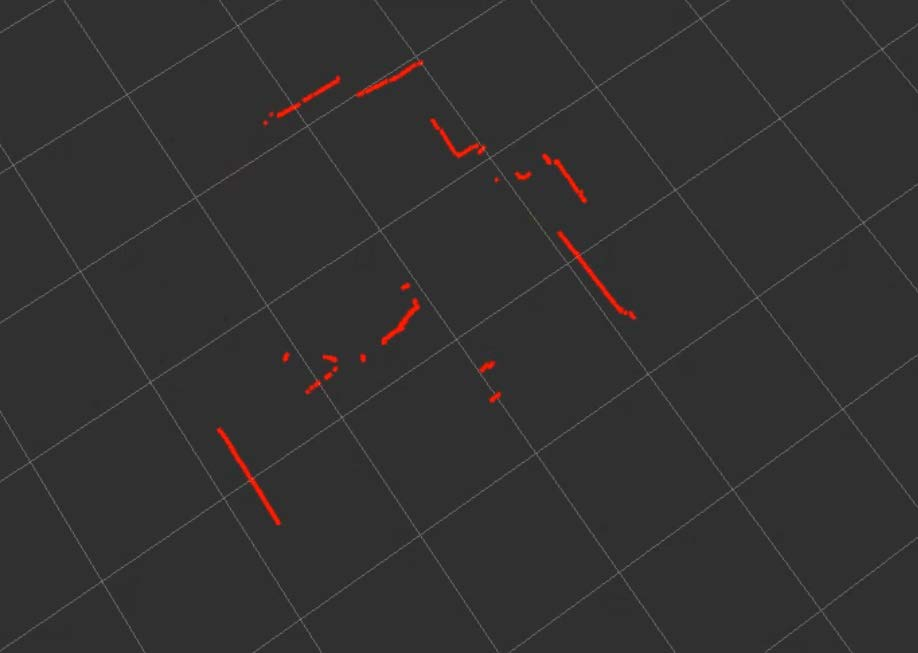
\includegraphics[scale=1.0]{lidar-2d}
    }
    \caption{Пример визуализации данных 2D LiDAR'а YDLiDAR X4}\label{fig:lidar-2d}
\end{figure}

\subsection{Альтернатива LiDAR}
В качестве альтернативы, предложенной в предыдущем пункте, можно рассмотреть иной способ получения информации об окружающем пространстве - использование камеры глубины. Одними из самых известных представителей являются камеры Xbox 360 Kinect, а также Intel RealSense Depth Camera D455, изображённые на Рисунке~\cref{fig:lidar-alts}~\cite{realsense,kinect-picture}.

\begin{figure}[ht]
    \centerfloat{
        \hfill
        \subcaptionbox[Intel® RealSense™ Depth Camera D455]{Внешний вид Intel® RealSense™ Depth Camera D455\label{fig:realsense}}{%
            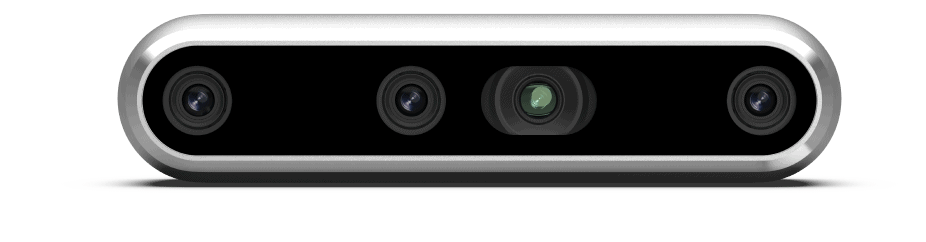
\includegraphics[width=0.5\linewidth]{realsense}}
        \hfill
        \subcaptionbox[Xbox 360 Kinect]{Внешний вид Xbox 360 Kinect\label{fig:kinect}}{%
            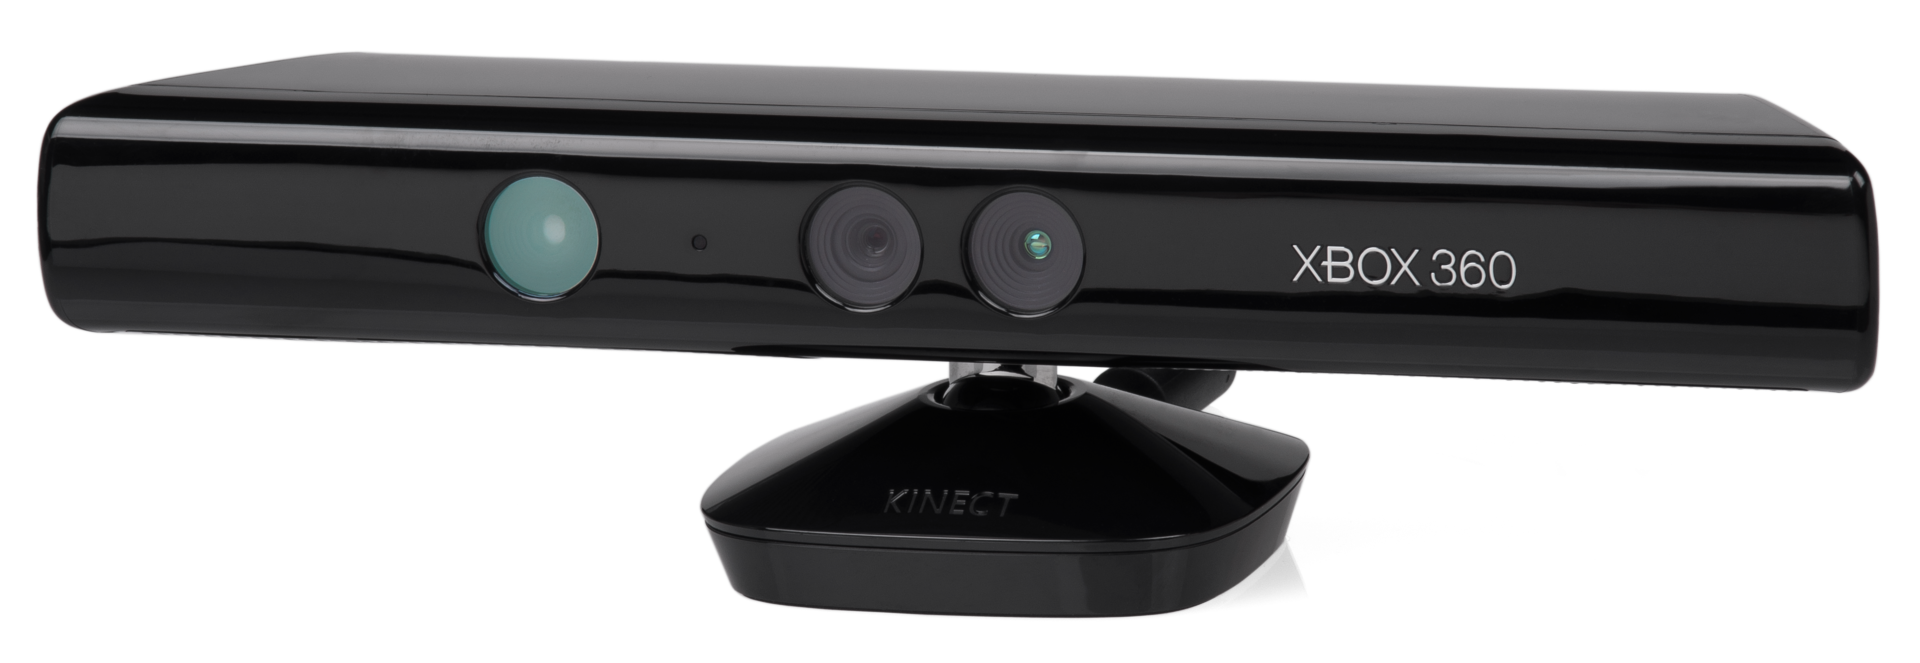
\includegraphics[width=0.5\linewidth]{kinect}}
        \hfill
    }
    \legend{}
    \caption[Камеры глубины]{Одни из самых известных камер глубины на рынке}\label{fig:lidar-alts}
\end{figure}

Камеры глубины в отличии от привычных видеокамер могут соотносить пиксели не только с цветом, но и с расстоянием до объекта в этой точке, как это показано на Рисунке~\cref{fig:depth-example}~\cite{depth-cameras}. К сожалению, данный способ получения информации об окружающем пространстве не позволит получать полную картину вокруг робота в следствии маленького угла обзора представленных камер сравнительно с лазерным сканером из предыдущего пункта данной работы.

\begin{figure}[ht]
    \centerfloat{
        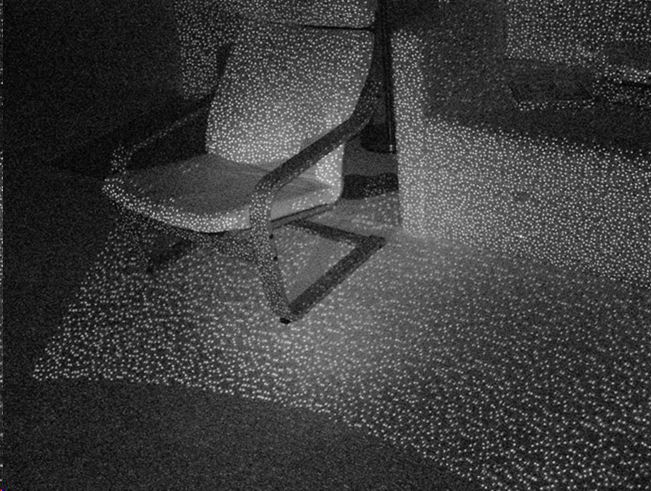
\includegraphics[scale=0.5]{depth-example}
    }
    \caption{Пример изображения с камеры глубины Xbox 360 Kinect.}\label{fig:depth-example}
\end{figure}

\subsection{Изображение с видеокамеры}
На компьютере NVIDIA Jetson Xavier NX, на котором будет работать нейросеть, существует два варианта подключения видеокамеры, которые будут рассмотрены в пунктах ниже.

\subsubsection{USB подключение}

Такой вариант подключения является самым популярным и без проблемным, так как на рынке имеется большое количество универсальных видеокамер с подключением по USB для любых целей. Для задач данной работы отлично подойдёт видеокамера Logitech C720 с разрешением видеосъёмки 1280x720 пикселей, изображённая на Рисунке~\cref{fig:usb-camera}~\cite{usb-camera}.

\begin{figure}[ht]
    \centerfloat{
        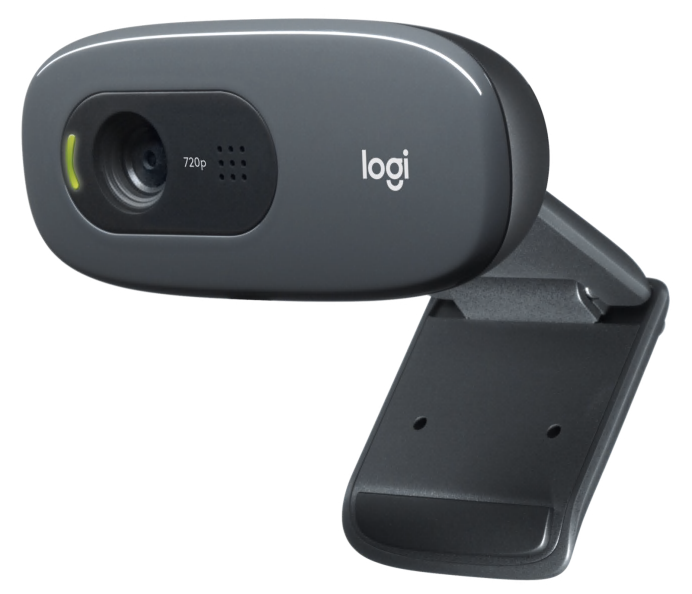
\includegraphics[scale=0.27]{usb-camera}
    }
    \caption{Внешний вид USB видеокамеры Logitech C720}\label{fig:usb-camera}
\end{figure}

\subsubsection{CSI подключение}

Данный способ подключения обладает как преимуществами, так и недостатками в сравнении с классическим USB подключением. Сравнительный анализ можно найти в Таблице~\cref{fig:usb-camera}~\cite{compare-csi-usb}.

\begin{table} [htbp]
    \centering
    \begin{threeparttable}% выравнивание подписи по границам таблицы
        \caption{Сравнение способов подключения видеокамеры к компьютеру NVIDIA Jetson Xavier NX}\label{tab:CameraCompare}%
        \begin{tabular}{| p{4cm} || p{6cm} | p{6cm}l |}
            \hline
            Рассматриваемый аспект       & \centering USB 3.0 подключение                                                 & \centering CSI подключение                                                     & \\
            \hline
            Доступность                              & \centering  Широкий выбор модельного ряда                             & \centering Единственная совместимая камера                     & \\
            \hline
            Ширина канала данных           & \centering  400 МБ/с                                                                       & \centering  320 МБ/с по одной линии (всего 4 линии)           & \\
            \hline
            Надёжность                              & \centering  USB порт, который относительно тяжело сломать & \centering Легко переламывающийся шлейф и коннектор & \\
            \hline
            Максимальная длина кабеля & \centering  Менее 5 метров                                                            & \centering  Менее 30 сантиметров                                          & \\
            \hline
            <<Горячее>> подключение    & \centering  Поддерживается                                                          & \centering  Не поддерживается                                              & \\
            \hline
            Габариты устройства              & \centering  Как правило, небольшие: 73x32x66 мм                      & \centering  Крошечный размер: 25x24x9 мм                          & \\
            \hline
        \end{tabular}
    \end{threeparttable}
\end{table}

Компьютер NVIDIA Jetson Xavier NX обладает совместимостью с единственной CSI камерой модели Sony IMX219, изображённая на Рисунке~\cref{fig:usb-camera}. Она оснащена 8 мегапиксельной матрицей с фокусным расстоянием 33 мм, а также имеет режим видеосъёмки в разрешении 1920x1080 пикселей с частотой кадров 30\footnote{1080p 30fps}~\cite{csi-camera}.

\begin{figure}[ht]
    \centerfloat{
        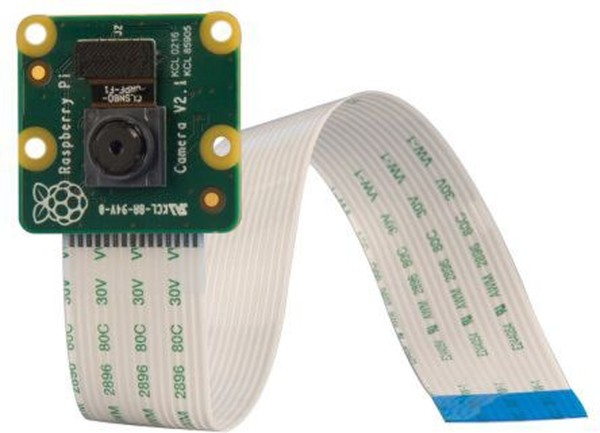
\includegraphics[scale=1.3]{csi-camera}
    }
    \caption{Внешний вид CSI видеокамеры Sony IMX219}\label{fig:csi-camera}
\end{figure}

По итогу сравнения, приоритет был дан на CSI подключение для ускорения обработки изображения, так как ресурсы мобильного компьютера сильно ограничены.

\section{Шасси робота}
Шасси робота определяет его <<мобильность>> и способность преодолевать различные препятствия. При выборе шасси необходимо искать компромиссы. С одной стороны, оно не должно быть большим, чтобы была возможность проезда в узких местах и не должно быть маленьким чтобы уместить всё оборудование на безопасном расстоянии друг от друга. 

В основной своей массе, по своей подвижной части шасси подразделяются на гусеничные и колёсные. Для робота было выбрано гусеничное шасси TS100, изображённое на Рисунке~\cref{fig:chassis}~\cite{chassis}. Такой выбор сделан чтобы отработать движения на гусеницах, которые более устойчивы к неровной поверхности дороги\footnote{В будущем предполагается использование робота в полевых условиях}.

\begin{figure}[ht]
    \centerfloat{
        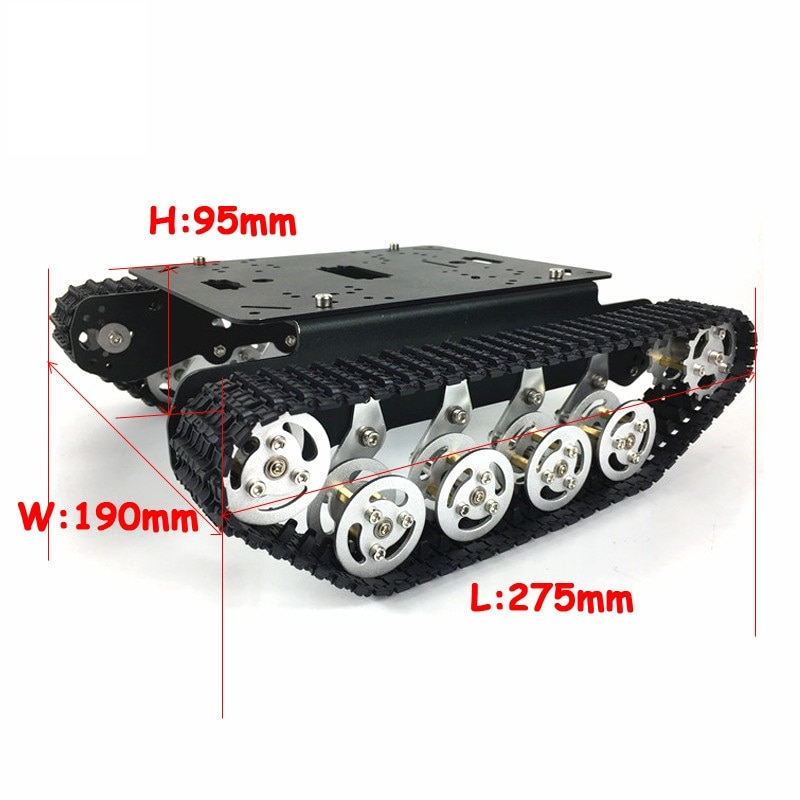
\includegraphics[scale=0.4]{chassis}
    }
    \caption{Внешний вид выбранного гусеничного шасси для робота TS100}\label{fig:chassis}
\end{figure}

Данное шасси имеет следующие характеристики~\cite{chassis}:
\begin{enumerate}[beginpenalty=10000] % https://tex.stackexchange.com/a/476052/104425
  \item Материал: алюминиевый сплав;
  \item Размер: 275x190x95 мм;
  \item Вес: 1100г.
\end{enumerate}

Шасси дополнительно укомплектовано двумя экземплярами электродвигателя DT25-370, которое изображено на Рисунке~\cref{fig:motor}~\cite{motor}.

\begin{figure}[ht]
    \centerfloat{
        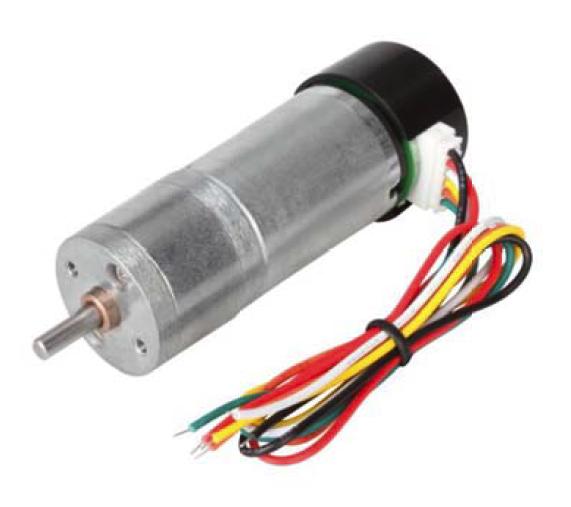
\includegraphics[scale=0.27]{motor}
    }
    \caption{Внешний вид электродвигателя DT25-370}\label{fig:motor}
\end{figure}

Двигатель имеет следующие характеристики~\cite{motor}:
\begin{enumerate}[beginpenalty=10000] % https://tex.stackexchange.com/a/476052/104425
  \item Максимальная скорость: 150 оборотов в минуту;
  \item Допустимая нагрузка: 3 кг;
  \item Рабочее напряжение: 9 вольт;
  \item Датчики Холла: 2 шт;
  \item Максимальное потребление тока: 4.5 А.
\end{enumerate}

\section{Рассмотрение аналогов}
К известным аналогам разрабатываемого робота, созданных на базе такой же платформы Jetson можно причислить роботов от самой компании NVIDIA: JetBot и Kaya. Оба эти робота были созданы для демонстрации возможностей одноплатного компьютера NVIDIA Jetson Nano.

\subsection{NVIDIA Kaya}
Данная модель компактного мобильного автономного робота была представлена на технологической конференции GTC 2019 и в первую очередь предназначается для работы с программным обеспечением Isaac SDK. Робот представлен на Рисунке~\cref{fig:kaya}.

\begin{figure}[ht]
    \centerfloat{
        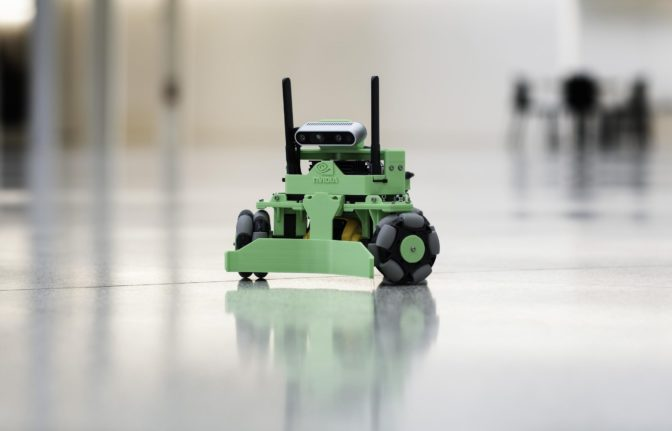
\includegraphics[scale=1.0]{kaya}
    }
    \caption{Внешний вид робота NVIDIA Kaya}\label{fig:kaya}
\end{figure}

Аппаратно данный робот помимо самого Jetson NANO включает в себя пластиковый корпус на трёх колёсах (печатаемый на 3D принтере), 3D камеру LiDAR Intel Real Sense и систему управления. Общая стоимость аппаратной части на момент написания данной работы\footnote{июнь 2022} составляет 812.87\$~\cite{kaya}.

На компьютер Jetson NANO помимо ОС Ubuntu 18.04 LTS устанавливается ПО Isaac SDK и Isaac SIM. Isaac SDK - это открытая платформа NVIDIA для интеллектуальных роботов. Она предоставляет большой набор мощных алгоритмов, базирующихся на GPU вычислениях\footnote{вычисления на видеокарте} для навигации и управления.

На данном роботе можно запускать различные готовые примеры такие как ручное управление с игрового контроллера Playstation 4, автономное следование
за AprilTag, распознавание объектов на нейронной сети DetectNetv2 и алгоритм SLAM (основан на GMapping)~\cite{isaac-kaya}.

\subsection{NVIDIA JetBot}

JetBot был представлен на той же конференции, что NVIDIA Kaya и является гораздо более доступным вариантом (цена 422.99\$ на момент написания работы) для создания DIY робота (также он в отличии от Kaya имеется в розничной продаже одним комплектом и его не нужно собирать по частям из разных магазинов). NVIDIA JetBot изображён на Рисунке~\cref{fig:jetbot}~\cite{jetbot}.

\begin{figure}[ht]
    \centerfloat{
        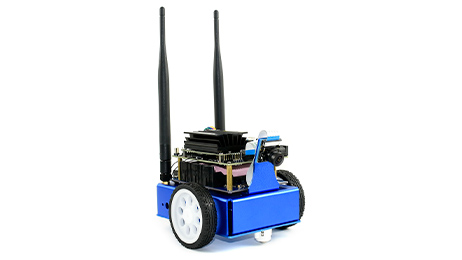
\includegraphics[scale=1.0]{jetbot}
    }
    \caption{Внешний вид робота NVIDIA JetBot}\label{fig:jetbot}
\end{figure}

Аппаратно он состоит из всё той же Nvidia Jetson Nano, двух электромоторов с драйвером в комплекте и CSI видеокамеры Sony IMX219. 

Программная часть поставляется готовым образом на базе Ubuntu 18.04 в формате ISO для прошивки MicroSD карты.

Из доступных примеров имеется простое ручное управление через кнопки на экране с возможностью прямой трансляции изображения видеокамеры на экран в браузере и автономное движение по поверхности с распознанием препятствий и пропастей в окружающем пространстве при помощи нейронной сети на основе получаемого видеосигнала. Также имеется функция следования робота за определённым целевым объектом~\cite{jetbot-examples}.

\FloatBarrier
